\documentclass[a4paper]{article}
\usepackage{graphicx} % Required for inserting images
\usepackage{indentfirst}
\usepackage[brazil]{babel}
\usepackage{amssymb}
\usepackage{amsmath}
\usepackage{dsfont}
\usepackage[left=2.5cm,top=2.5cm,right=2.5cm,bottom=2.5cm]{geometry}
\usepackage{tikz}
\usepackage{float}
\usepackage{multirow}
\graphicspath{ {./images/} }

\title{Métodos de Monte Carlo utilizando números Quasi-aleatórios - MAP2212}
\author{Antonio Gabriel Freitas da Silva - 13687290}
\date{Maio 2023}

\begin{document}

\maketitle

\section{Introdução}

A geração de números aleatórios verdadeiros pode ser difícil e muitas vezes requer muito tempo e recursos computacionais. Por essa razão, foram desenvolvidos os chamados números quasi-aleatórios, que são sequências de números que possuem algumas propriedades semelhantes às sequências aleatórias, mas que podem ser geradas de forma determinística e eficiente. O objetivo deste trabalho é justamente fazer a estimação da integral da função $f(x) = \exp{(-0.32798830x)}\cdot\cos{(0.04715069237x)}$ no intervalo $[0,1]$ utilizanfo os m;etodos de geração de pontos quasi-aleatórios e comparar com o método anterior.

\section{Comparação entre a geração de amostras e convergência das integrais}

Os números quasi-aleatórios, também conhecidos como números pseudo-aleatórios de baixa discrepância, são uma alternativa aos geradores de números pseudo-aleatórios tradicionais na simulação de Monte Carlo. Eles são gerados a partir de sequências determinísticas e repetitivas, com uma distribuição uniforme em um intervalo unitário. Essas sequências apresentam uma dispersão muito menor que as sequências geradas pelos geradores pseudo-aleatórios tradicionais, permitindo uma cobertura mais uniforme do espaço de amostragem.

Os números quasi-aleatórios têm vantagens em algumas aplicações, principalmente em problemas de alta dimensionalidade, onde o número de amostras necessárias para uma boa convergência é muito grande. Eles também são úteis para reduzir a variância do estimador em problemas de Monte Carlo. No entanto, em alguns casos, a utilização de números quasi-aleatórios pode ser pior em termos de tempo computacional, especialmente em problemas de baixa dimensionalidade, onde os geradores pseudo-aleatórios são mais eficientes.

Para fins práticos, será usada as sequências de Halton, que é baseado em uma série de bases primas, que são números primos relativamente próximos, que são usados para gerar uma sequência de pontos em um espaço de dimensão alta. Cada ponto dessa sequência tem uma distribuição uniforme, e a distribuição conjunta de todos os pontos se aproxima de uma distribuição uniforme em todo o espaço.
 O método de Halton é um dos métodos mais populares e amplamente utilizados para gerar sequências quasi-aleatórias, devido à sua facilidade de implementação, eficiência computacional e melhor cobertura do espaço em dimensões mais altas. 

 Os métodos de quasi-Monte Carlo, incluindo o método Halton, são projetados para ter uma baixa discrepância, o que significa que seus pontos amostrais são distribuídos mais uniformemente do que amostras aleatórias. Isso permite uma melhor convergência para estimar a integral em comparação com as amostras aleatórias.

No entanto, a convergência ainda depende da função a ser integrada e da dimensão do espaço de integração. Para funções suaves em dimensões de baixa a moderada (até cerca de 20 dimensões), o método dos quasi-aleatórios pode levar a uma convergência mais rápida do que o método de Monte Carlo com amostras aleatórias. No entanto, para funções irregulares em dimensões mais altas, a convergência pode não ser tão boa e o método de Monte Carlo com amostras aleatórias pode ser mais eficaz. Logo, o tempo computacional neste programa teve uma piora em relação aos métodos pseudo-aleatórios.

\begin{figure}[H]
  \centering
  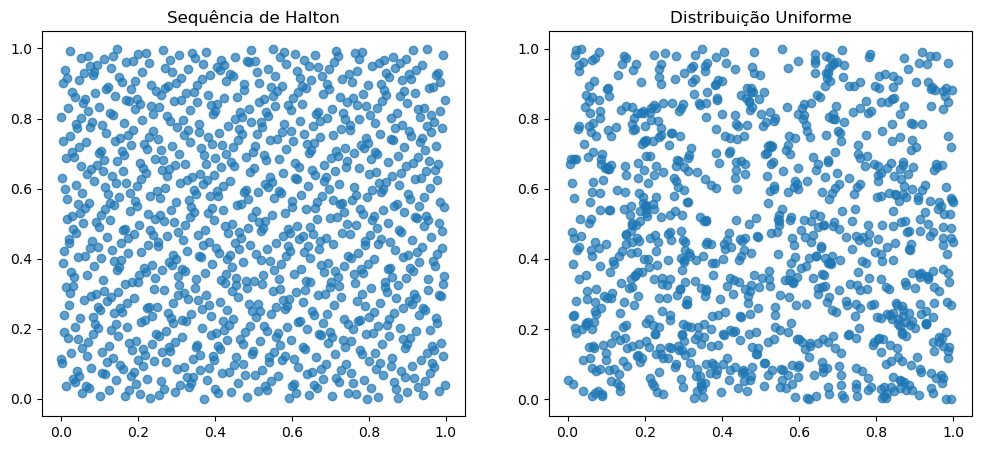
\includegraphics[width=0.7\textwidth]{HxU.png}
  \caption{Comparação entre a dispersão de 1000 pontos quasi-aleatórios e distribuição uniforme}
  \label{fig:HxU}
\end{figure}

Em compensação, existe uma melhora de Halton com relação a integral estimada, o QMC está mais bem-estimada que o PRNG como podemos ver abaixo:

\begin{figure}[H]

  \centering
  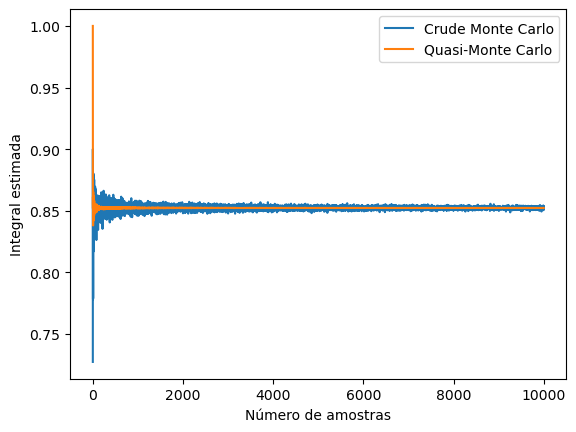
\includegraphics[width=0.4\textwidth]{Crude.png}
  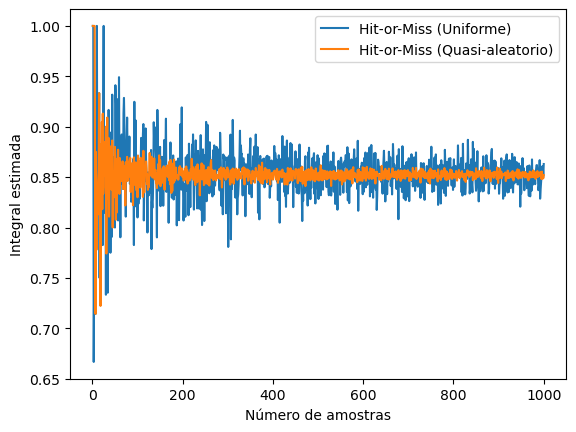
\includegraphics[width=0.4\textwidth]{HM.png}
  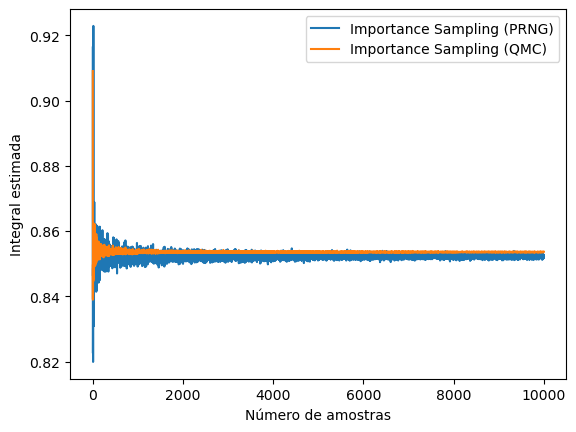
\includegraphics[width=0.4\textwidth]{IS.png}
  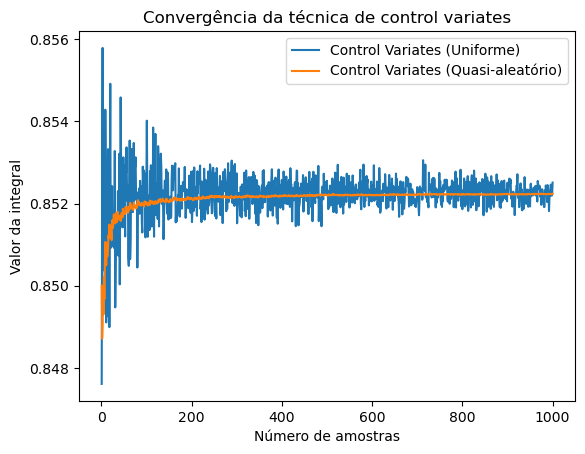
\includegraphics[width=0.4\textwidth]{CV.png}
  \caption{Comparação entre cada método utilizando a amostragem pseudo-aleatórias e quasi-aleatórias (10000 pontos no Crude e Importance Sampling e 1000 nos demais).}
\end{figure}

\section{Exemplo de simulação e Conclusão}
Abaixo, podemos ver como os programa se comportam com uma Seed de 12643601, ao distribuir 10000 pontos:

\begin{table}[h]
\centering
\begin{tabular}{|l|c|c|c|c|c|}
\hline
Método & Integral estimada PRNG & Tempo (s) & Integral estimada QMC & Tempo (s) \\
\hline
Crude & 0.851599 & 0.000208 & 0.852314 & 0.000409  \\
\hline
Hit or Miss & 0.850000 & 0.049711 & 0.853600 & 0.020757 \\
\hline
Importance Sampling & 0.852173 & 0.001445 & 0.853467 & 0.002733 \\
\hline
Control Variates & 0.852191 & 0.047804 & 0.852262 & 0.149104\\
\hline
\end{tabular}
\caption{Tabela de resultados dos métodos de integração.}
\label{tab:resultados}
\end{table}

Logo, percebemos uma melhora melhor no Hit or Miss, enquanto que a maior piora foi no método de Control Variates.

Concluindo, foi destacada a diferença entre a amostragem aleatória por números pseudoaleatórios e por números quasi-aleatórios. Enquanto a primeira é amplamente utilizada por ser fácil de implementar e por possuir propriedades estatísticas adequadas, a segunda apresenta vantagens em algumas situações, como a convergência mais rápida da estimativa e menor variância.

Por fim, pode ser ressaltado que a escolha do método adequado depende das características do problema em questão e que, em muitos casos, a combinação de técnicas pode levar a estimativas ainda mais precisas. Além disso, o tempo computacional é um fator importante a ser considerado, e a escolha do método deve levar em conta também a disponibilidade de recursos computacionais.

\end{document}
